% \documentclass[mathserif, serif]{beamer}
\documentclass[xetex, mathserif, serif]{beamer}
% \usepackage[utf8]{fontenc}
% 
% The default font in XeLaTeX doesn't have the default bullet character, so 
% either change the font:
% \setmainfont{XITS}
% \setmathfont{XITS Math}
% 
% Or change the character:
% \setbeamertemplate{itemize items}{•}

\setbeamertemplate{footline}[frame number]
\setbeamertemplate{navigation symbols}{}
\usepackage{amsmath}
\usepackage{amssymb}
\usepackage{bm}
\bibliographystyle{apalike}
\setbeamerfont{bibliography item}{size=\scriptsize}
\setbeamerfont{bibliography entry author}{size=\scriptsize}
\setbeamerfont{bibliography entry title}{size=\scriptsize}
\setbeamerfont{bibliography entry location}{size=\scriptsize}
\setbeamerfont{bibliography entry note}{size=\scriptsize}

\setbeamertemplate{blocks}[rounded][shadow=false]
\setbeamertemplate{itemize item}[circle]
\setbeamertemplate{itemize subitem}[circle]
\setbeamercolor{block body}{bg=blue!10!white}
\setbeamercolor{block body example}{fg=black!100, bg=black!10!white}
\setbeamercolor{block title example}{fg=black!70, bg=black!10!white}
\newenvironment{idea}
{
  \begin{block}{}
    \begin{columns}
      % \begin{column}{.001\textwidth}
      % \end{column}
      \begin{column}{.04\textwidth}
        $\qquad\qquad$
          \includegraphics[scale=.05]{img/idea}
      \end{column}
      \begin{column}{.9\textwidth}
  }
  {
  \end{column}
\end{columns}
  \end{block}
}

\usepackage[T1]{fontenc}
\usepackage{lmodern}

\usepackage{tikz-cd}
\usetikzlibrary{backgrounds}
\usetikzlibrary{arrows}

\usepackage{tikz}
\usepackage{bm}
\usepackage[absolute,overlay]{textpos}
\usepackage{cancel}


\usepackage{algorithm}
\usepackage[noEnd=True, indLines=True]{algpseudocodex}
\algrenewcommand\algorithmicrequire{\textbf{Input:}}
\algrenewcommand\algorithmicensure{\textbf{Output:}}

\newcommand{\backupbegin}{
  \newcounter{finalframe}
  \setcounter{finalframe}{\value{framenumber}}
}
\newcommand{\backupend}{
  \setcounter{framenumber}{\value{finalframe}}
}

\newcommand{\mdef}{:=}
% \newcommand{\mname}[1]{\textit{{#1}}}
\newcommand{\mname}[1]{\underline{{#1}}}
\renewcommand{\problem}[1]{\textsc{{#1}}}
\newcommand{\mlist}[1]{[ {#1} ]}

\newcommand{\join}{\wedge}
\newcommand{\meet}{\vee}
\newcommand{\dedekind}{\square_{\join \meet}}
% \newcommand{\pint}{[1]}
\newcommand{\pint}[1]{\mathbf{I}^{#1}}
\newcommand{\pintrestr}[3]{\mathbf{I}^{#1}_{{#2}={#3}}}
% \newcommand{\izero}{\mathsf{0}}
% \newcommand{\ione}{\mathsf{1}}
\newcommand{\izero}{{\scriptstyle\mathbf{0}}}
\newcommand{\ione}{{\scriptstyle\mathbf{1}}}
\newcommand{\ivar}{*}
\newcommand{\restrict}[2]{{#1}|_{#2}}
\newcommand{\image}[1]{\textsf{Img}({#1})}
\newcommand{\psh}[1]{\mathbf{Set}^{{#1}^{op}}}
\renewcommand{\hom}[2]{\text{Hom}({#1} , {#2})}
\renewcommand{\dim}[1]{\mathsf{dim}({#1})}
\newcommand{\ctxtdim}[1]{|{#1}|}
\newcommand{\smap}[1]{s^{{#1}}}
\newcommand{\dmap}[2]{d^{({#1} , {#2})}}
% \newcommand{\cont}[2]{{#1}\langle{#2}\rangle}
\newcommand{\cont}[2]{ \ifthenelse{\equal{#2}{}}{#1}{{#1}\langle{#2}\rangle} }

\newcommand{\pow}[1]{\mathcal{P}({#1})}
\newcommand{\cset}[1]{\ensuremath{\mathsf{{#1}}}}
\newcommand{\boundary}[1]{\partial({#1})}
\newcommand{\comp}[2]{\mathsf{Comp}({#1}\ {#2})}


\newcommand{\pc}{\cdot}
\newcommand{\pcfill}[2]{\ensuremath{\pc\cset{fill}_{{#1},{#2}}}}
\newcommand{\inv}[1]{{#1}^{-1}}
\newcommand{\invfill}[1]{\ensuremath{\inv{#1}\cset{fill}}}

\newcommand{\substtwo}[2]{\tiny
  \arraycolsep=.4pt\def\arraystretch{1}
  \begin{array}{ll}
    0 &\mapsto {#1} \\
    1 &\mapsto {#2}
  \end{array}
}
% \newcommand{\oneconst}{\substtwo{()}{()}}
\newcommand{\oneconst}{s^1}
\newcommand{\oneid}{\substtwo{0}{1}}

\newcommand{\substfour}[4]{\tiny
  \arraycolsep=.4pt\def\arraystretch{1}
  \begin{array}{ll}
    00 &\mapsto {#1} \\
    01 &\mapsto {#2} \\
    10 &\mapsto {#3} \\
    11 &\mapsto {#4} 
  \end{array}
}

\newcommand{\appfstsubst}{\substfour{0}{0}{1}{1}}
\newcommand{\appsndsubst}{\substfour{0}{1}{0}{1}}
\newcommand{\orsubst}{\substfour{0}{1}{1}{1}}
\newcommand{\andsubst}{\substfour{0}{0}{0}{1}}

\newcommand{\substfourlarge}[4]{\small
  \arraycolsep=.4pt\def\arraystretch{1}
  \begin{array}{ll}
    00 &\mapsto {#1} \\
    01 &\mapsto {#2} \\
    10 &\mapsto {#3} \\
    11 &\mapsto {#4} 
  \end{array}
}

\newcommand{\dimcube}[3]{
  \begin{tikzpicture}[scale=0.3]
    \draw[->,>=stealth] (0,0) -- (0,1) node [near end,right, fill=none] {$#1$};
    \draw[->,>=stealth] (0,0) -- (1,0) node [near end,below, fill=none] {$#2$};
    \draw[->,>=stealth] (0,0) -- (-.71,-.71) node [near end,above=.02cm, fill=none] {$#3$};
  \end{tikzpicture}
}


\newcommand{\dimsquare}[2]{
  \begin{tikzpicture}[scale=0.30]
    \draw[->,>=stealth] (0,0) -- (1,0) node [near end,below, fill=none] {$#1$};
    \draw[->,>=stealth] (0,0) -- (0,1) node [near end,left, fill=none] {$#2$};
  \end{tikzpicture}
}

\newcommand{\filledsquare}[5]{
  \begin{tikzpicture}[scale=.5]
    \draw[->,>=stealth] (0,0) -- (3,0) node [midway,below, fill=none] {\ensuremath{#1}};
    \draw[->,>=stealth] (0,3) -- (3,3) node [midway,above, fill=none] {\ensuremath{#2}};
    \draw[->,>=stealth] (0,0) -- (0,3) node [midway,left,  fill=none] {\ensuremath{#3}};
    \draw[->,>=stealth] (3,0) -- (3,3) node [midway,right, fill=none] {\ensuremath{#4}};
    \node [fill=none] at (1.5, 1.5) {\ensuremath{#5}};
  \end{tikzpicture}
}

\newcommand{\hcompcube}[9]{
  \begin{tikzpicture}[scale=.85]
    \draw[->,>=stealth] (0,0) -- (4,0) node [midway,below, fill=none] {\ensuremath{#1}};
    \draw[->,>=stealth] (0,4) -- (4,4) node [midway,above, fill=none] {\ensuremath{#2}};
    \draw[->,>=stealth] (0,0) -- (0,4) node [midway,left=.2cm, fill=none] {\ensuremath{#3}};
    \draw[->,>=stealth] (4,0) -- (4,4) node [midway,right=.2cm,fill=none] {\ensuremath{#4}};

    \draw[->,>=stealth] (1.2,1.2) -- (2.8,1.2);
    \draw[->,>=stealth] (1.2,1.2) -- (1.2,2.8);
    \draw[->,>=stealth] (2.8,1.2) -- (2.8,2.8);
    \draw[->,>=stealth] (1.2,2.8) -- (2.8,2.8);

    \draw[->,>=stealth] (1.2,1.2) -- (0,0);
    \draw[->,>=stealth] (2.8,1.2) -- (4,0);
    \draw[->,>=stealth] (2.8,2.8) -- (4,4);
    \draw[->,>=stealth] (1.2,2.8) -- (0,4);

    \node at (2, .6)  {\ensuremath{#5}};
    \node at (2, 3.4) {\ensuremath{#6}};
    \node at (.6, 2)  {\ensuremath{#7}};
    \node at (3.4, 2) {\ensuremath{#8}};
    \node at (2, 2)  {\ensuremath{#9}};
  \end{tikzpicture}
}


% \newcommand{\hcompcube}[9]{
%   \begin{tikzpicture}[scale=.8]
%     \draw[->,>=stealth] (0,0) -- (4,0) node [midway,below, fill=none] {\ensuremath{#1}};
%     \draw[->,>=stealth] (0,0) -- (0,4) node [midway,left=.2cm, fill=none] {\ensuremath{#2}};
%     \draw[->,>=stealth] (0,4) -- (4,4) node [midway,above, fill=none] {\ensuremath{#3}};
%     \draw[->,>=stealth] (4,0) -- (4,4) node [midway,right=.2cm,fill=none] {\ensuremath{#4}};

%     \draw[->,>=stealth] (1,1) -- (3,1);
%     \draw[->,>=stealth] (1,1) -- (1,3);
%     \draw[->,>=stealth] (3,1) -- (3,3);
%     \draw[->,>=stealth] (1,3) -- (3,3);

%     \draw[->,>=stealth] (1,1) -- (0,0);
%     \draw[->,>=stealth] (3,1) -- (4,0);
%     \draw[->,>=stealth] (3,3) -- (4,4);
%     \draw[->,>=stealth] (1,3) -- (0,4);

%     \node at (2, .5)  {\ensuremath{#5}};
%     \node at (.5, 2)  {\ensuremath{#6}};
%     \node at (2, 3.5) {\ensuremath{#7}};
%     \node at (3.5, 2) {\ensuremath{#8}};
%     \node at (2, 2)  {\ensuremath{#9}};
%   \end{tikzpicture}
% }

\newcommand{\hcompcubesmall}[9]{
  \begin{tikzpicture}[scale=.8]
    \draw[->,>=stealth] (0,0) -- (4,0) node [midway,below, fill=none] {\ensuremath{#1}};
    \draw[->,>=stealth] (0,0) -- (0,4) node [midway,left=.2cm, fill=none] {\ensuremath{#2}};
    \draw[->,>=stealth] (0,4) -- (4,4) node [midway,above, fill=none] {\ensuremath{#3}};
    \draw[->,>=stealth] (4,0) -- (4,4) node [midway,right=.2cm,fill=none] {\ensuremath{#4}};

    \draw[->,>=stealth] (1,1) -- (3,1);
    \draw[->,>=stealth] (1,1) -- (1,3);
    \draw[->,>=stealth] (3,1) -- (3,3);
    \draw[->,>=stealth] (1,3) -- (3,3);

    \draw[->,>=stealth] (1,1) -- (0,0);
    \draw[->,>=stealth] (3,1) -- (4,0);
    \draw[->,>=stealth] (3,3) -- (4,4);
    \draw[->,>=stealth] (1,3) -- (0,4);

    \node at (2, .5)  {\ensuremath{#5}};
    \node at (.5, 2)  {\ensuremath{#6}};
    \node at (2, 3.5) {\ensuremath{#7}};
    \node at (3.5, 2) {\ensuremath{#8}};
    \node at (2, 2)  {\ensuremath{#9}};
  \end{tikzpicture}
}

\title{\hspace{-.7em}Automating reasoning in cubical type theory\vspace{1em}}
\subtitle{EPN WG 6 meeting\\\textit{Vienna, 25 April 2023}}
\author{Maximilian Dor\'e\\\url{maximilian.dore@cs.ox.ac.uk}} \date{}

\begin{document}

\maketitle



\begin{frame}
  \frametitle{Motivation}

  \begin{itemize}
  \item Cubical Agda introduces new kind of proof obligation: given a boundary in a
    Kan cubical set, construct a cell with that boundary.
  \item Explore interval substitutions and Kan compositions as principles of
    logic

    $\to$ Automate higher equational reasoning 
  \end{itemize}

\end{frame}


% \begin{frame}
%   \frametitle{Higher inductive types and interval substitutions}

%   In Cubical Agda, higher inductive types generate cubical sets.

%   \begin{exampleblock}{}
%     \begin{columns}
%       \begin{column}{.6\textwidth}
%     \textbf{data} \cset{Circle} \textbf{where}
%     \begin{itemize}
%     \item $\cset{base} : \cset{Circle}$
%     \item $\cset{loop} : \cset{base} = \cset{base}$
%     \end{itemize}
%   \end{column}
%   \begin{column}{.3\textwidth}
%     \begin{tikzpicture}[scale=0.8]
%       \node (z) at (2.6,.7) {\cset{base}};
%       \node (o) at (2.6,-.7) {\cset{base}};
%       \draw[->,>=stealth] (o) -- (z) node[midway,right] {\cset{loop}};
%     \end{tikzpicture}
%   \end{column}
% \end{columns}
%   \end{exampleblock}

%   Cells can be contorted with interval substitutions: Abstracting over interval
%   variables drags
%   out a cube, application of formulas to cells prescribe the boundary of the
%   produced cube.
%   % \begin{itemize}
%   % \item \emph{abstract} over interval variables
%   % \item \emph{apply} elements of lattice over interval variables
%   % \end{itemize}

%   \begin{exampleblock}{}
%     $\lambda\ i\ j \to \cset{loop}\ (i \vee j)$

%     $\qquad: \mathsf{PathP}\ (\lambda i \to \mathsf{Path}\ \mathsf{Circle}\
%     (\mathsf{loop}\ i)\ \mathsf{base})\ \mathsf{loop}\ (\lambda j \to \mathsf{base})$
%   \end{exampleblock}
% \end{frame}


% \begin{frame}
%   \frametitle{Making sense of interval substitutions}

%   \begin{exampleblock}{}
%     $\lambda\ i\ j \to \cset{loop}\ (i \vee j)$
%   \end{exampleblock}

%   \vspace{1em}

%     \begin{columns}
%       \begin{column}{.3\textwidth}
%         \begin{tabular}{ l | l || c }
%           $i$ & $j$ & $i \vee j$ \\ \hline\hline
%           0 & 0 & 0 \\ \hline
%           0 & 1 & 1 \\ \hline
%           1 & 0 & 1 \\ \hline
%           1 & 1 & 1
%         \end{tabular}
%       \end{column}

%     \begin{column}{.4\textwidth}
%       \begin{tikzpicture}
%         % \node (zz) at (0,1) {\textcolor{gray}{00} $\mapsto \{x\}$};
%         % \node (zo) at (-1,0) {\textcolor{gray}{01} $\mapsto \{x , y\}$};
%         % \node (oz) at (1,0) {\textcolor{gray}{10} $\mapsto \{x , y\}$};
%         % \node (oo) at (0,-1) {\textcolor{gray}{11} $\mapsto \{y\}$};
%         \node (zz) at (0,1) {\textcolor{gray}{00}};
%         \node (zo) at (-1,0) {\textcolor{gray}{01}};
%         \node (oz) at (1,0) {\textcolor{gray}{10}};
%         \node (oo) at (0,-1) {\textcolor{gray}{11}};
%         \draw (zz) -- (zo) -- (oo) -- (oz) -- (zz);
%         % \end{tikzpicture}
%         % \begin{tikzpicture}[scale=1]
%           \node (z) at (2.6,.7) {\cset{base}};
%           \node (o) at (2.6,-.7) {\cset{base}};
%           \draw (z) -- (o) node[midway,right] {\cset{loop}};

%           \draw[|->] (zz) -- (z);
%           \draw[|->] (zo) -- (o);
%           \draw[|->] (oz) -- (o);
%           \draw[|->] (oo) -- (o);
%       \end{tikzpicture}
%     \end{column}
%   \end{columns}

%   TODO FIRST 0, 1 on the right and then overlay with definition?

%   TODO ANNOTATE EDGES IN SQUARE?

% \end{frame}




\begin{frame}
  \frametitle{Higher inductive types and interval substitutions}

  In Cubical Agda, higher inductive types generate cubical sets.

  \begin{exampleblock}{}
    \begin{columns}
      \begin{column}{.7\textwidth}
        \textbf{data} \cset{Sphere} \textbf{where}
        \begin{itemize}
        \item $\cset{base} : \cset{Sphere}$
        \item $\cset{surf} : \mathsf{Path}\ (\mathsf{Path}\
          \cset{Sphere}\ \cset{base}\ \cset{base})\ \mathsf{refl}\ \mathsf{refl}$

          % TODO PathP Notation ok here?
        \end{itemize}
      \end{column}
      \begin{column}{.2\textwidth}
        \vspace{-.8em} \filledsquare{}{}{}{}{\cset{surf}} \vspace{-1.5em}
      \end{column}
    \end{columns}
  \end{exampleblock}

  Cells can be contorted with interval substitutions: Abstracting over interval
  variables drags
  out a cube, application of formulas to cells prescribe the boundary of the
  produced cube.
  % \begin{itemize}
  % \item \emph{abstract} over interval variables
  % \item \emph{apply} elements of lattice over interval variables
  % \end{itemize}

  \begin{exampleblock}{}
    $\lambda\ i\ j\ k \to \cset{surf}\ (i \vee k)\ ((i \wedge j) \vee k))$

    $\quad : \mathsf{PathP} (\lambda i \to \mathsf{PathP} (\lambda j \to
    \mathsf{Path}\ \mathsf{Sphere}$

    $\qquad (\cset{surf}\ i\ (i \wedge j))\ \cset{base})$

    $\qquad (\lambda k \to \cset{surf}\ (i \vee k)\ k)\ (\lambda k \to \cset{surf}\ (i \vee k)\ (i \vee k)))$

    $\qquad(\lambda j\ k \to \cset{surf}\ k\ k)\ (\lambda j\ k \to \cset{base})$

    % $\quad: \mathsf{PathP}\ (\lambda i \to \mathsf{Path}\ \mathsf{Circle}\
    % (\mathsf{loop}\ i)\ \mathsf{base})\ \mathsf{loop}\ (\lambda j \to \mathsf{base})$
  \end{exampleblock}
\end{frame}







\begin{frame}
  \frametitle{Interval substitutions as poset maps}

  \begin{exampleblock}{}
    \begin{columns}
      \begin{column}{.7\textwidth}
        \textbf{data} \cset{Sphere} \textbf{where}
        \begin{itemize}
        \item $\cset{base} : \cset{Sphere}$
        \item $\cset{surf} : \mathsf{Path}\ (\mathsf{Path}\
          \cset{Sphere}\ \cset{base}\ \cset{base})\ \mathsf{refl}\ \mathsf{refl}$

          % TODO PathP Notation ok here?
        \end{itemize}
      \end{column}
      \begin{column}{.2\textwidth}
        \vspace{-.8em} \filledsquare{}{}{}{}{\cset{surf}} \vspace{-1.5em}
      \end{column}
    \end{columns}
    $\lambda\ i\ j\ k \to \cset{surf}\ (i \vee k)\ ((i \wedge j) \vee k))$
  \end{exampleblock}

    \begin{columns}
      \begin{column}{.3\textwidth}
        \bgroup
        \def\arraystretch{1.2}
        \setlength\tabcolsep{.2em}
        \tiny
        \begin{tabular}{ l | l | l || c | c }
          $i$ & $j$ & $k$ & $i \vee k$ & $(i \wedge j) \vee k$ \\ \hline\hline
          \color<2>{red}{0} & \color<2>{red}{0} & \color<2>{red}{0} & \color<2>{red}{0} & \color<2>{red}{0} \\ \hline
          \color<2>{red}{0} & \color<2>{red}{0} & \color<2>{red}{1} & \color<2>{red}{1} & \color<2>{red}{1} \\ \hline
          \color<2>{red}{0} & \color<2>{red}{1} & \color<2>{red}{0} & \color<2>{red}{0} & \color<2>{red}{0} \\ \hline
          \color<2>{red}{0} & \color<2>{red}{1} & \color<2>{red}{1} & \color<2>{red}{1} & \color<2>{red}{1} \\ \hline
          \color<3->{red}{1} & \color<3->{red}{0} & \color<3->{red}{0} & \color<3->{red}{1} & \color<3->{red}{0} \\ \hline
          \color<3->{red}{1} & \color<3->{red}{0} & \color<3->{red}{1} & \color<3->{red}{1} & \color<3->{red}{1} \\ \hline
          \color<3->{red}{1} & \color<3->{red}{1} & \color<3->{red}{0} & \color<3->{red}{1} & \color<3->{red}{1} \\ \hline
          \color<3->{red}{1} & \color<3->{red}{1} & \color<3->{red}{1} & \color<3->{red}{1} & \color<3->{red}{1}
        \end{tabular}
        \egroup
      \end{column}

    \begin{column}{.7\textwidth}
      \only<1>{
        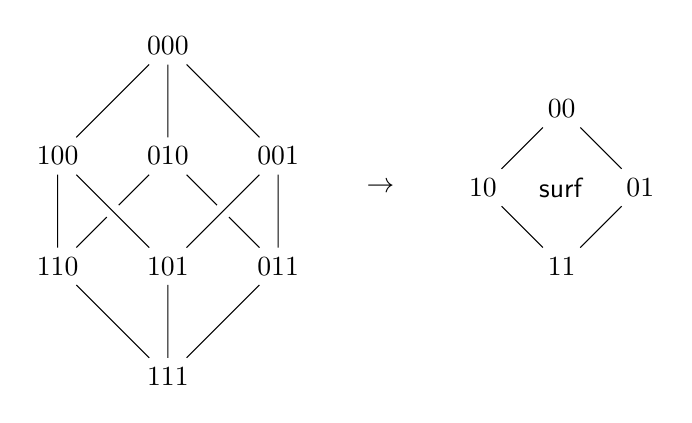
\begin{tikzpicture}
          \node (zzz) at (0,2.8) {$000$};
          \node (ozz) at (-1.4,1.4) {$100$};
          \node (zoz) at (0,1.4) {$010$};
          \node (ooz) at (-1.4,0) {$110$};
          \node (zzo) at (1.4,1.4) {$001$};
          \node (ozo) at (0,0) {$101$};
          \node (zoo) at (1.4,0) {$011$};
          \node (ooo) at (0,-1.4) {$111$};
          \draw (ooo) -- (ooz) -- (ozz) -- (zzz) -- (zoz) -- (zoo)
          (ozo) -- (ooo) -- (zoo) -- (zzo) -- (zzz)
          (ooz) -- (zoz);
          \draw[preaction={draw=white, -,line width=6pt}] (ozz) -- (ozo) -- (zzo);

          \begin{scope}[shift={(5,1)}]
            \node (zz) at (0,1) {00};
            \node (zo) at (-1,0) {10};
            \node (oz) at (1,0) {01};
            \node (oo) at (0,-1) {11};
            \node (filler) at (0,0) {\cset{surf}};
            \draw (zz) -- (zo) -- (oo) -- (oz) -- (zz);
          \end{scope}

          \node (filler) at (2.7,1) {$\to$};
        \end{tikzpicture}
      }

      \only<2>{
        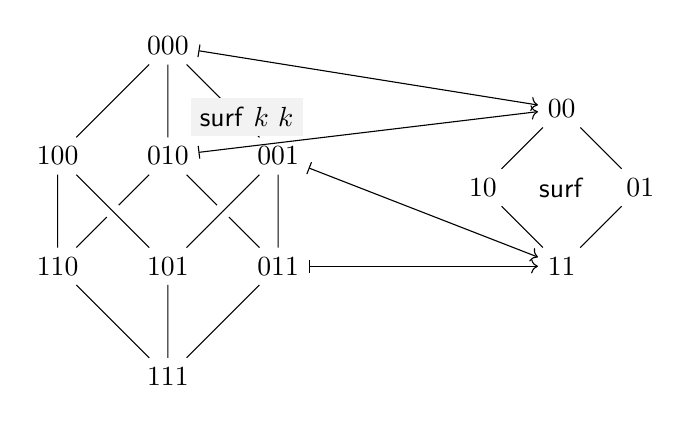
\begin{tikzpicture}
          \node (zzz) at (0,2.8) {$000$};
          \node (ozz) at (-1.4,1.4) {$100$};
          \node (zoz) at (0,1.4) {$010$};
          \node (ooz) at (-1.4,0) {$110$};
          \node (zzo) at (1.4,1.4) {$001$};
          \node (ozo) at (0,0) {$101$};
          \node (zoo) at (1.4,0) {$011$};
          \node (ooo) at (0,-1.4) {$111$};
          \draw (ooo) -- (ooz) -- (ozz) -- (zzz) -- (zoz) -- (zoo)
          (ozo) -- (ooo) -- (zoo) -- (zzo) -- (zzz)
          (ooz) -- (zoz);
          \draw[preaction={draw=white, -,line width=6pt}] (ozz) -- (ozo) -- (zzo);

          \begin{scope}[shift={(5,1)}]
            \node (zz) at (0,1) {00};
            \node (zo) at (-1,0) {10};
            \node (oz) at (1,0) {01};
            \node (oo) at (0,-1) {11};
            \node (filler) at (0,0) {\cset{surf}};
            \draw (zz) -- (zo) -- (oo) -- (oz) -- (zz);
          \end{scope}

          \draw[|->] (zzz) -- (zz);
          \draw[|->] (zzo) -- (oo);
          \draw[|->] (zoz) -- (zz);
          \draw[|->] (zoo) -- (oo);

          \node[fill=gray!10] (filler) at (1,1.9) {$\cset{surf}\ k\ k$};
        \end{tikzpicture}
      }

      \only<3->{
        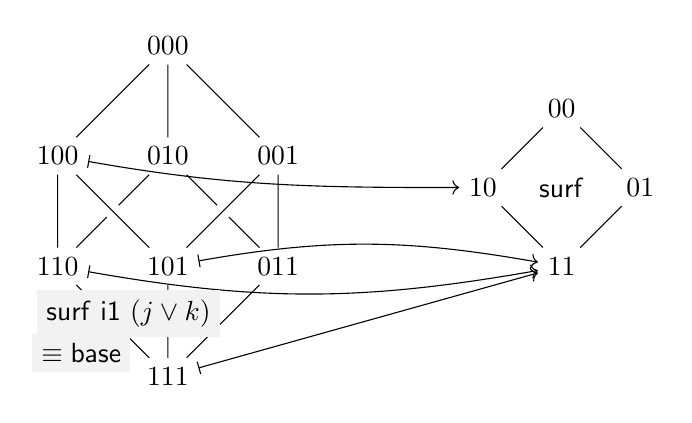
\begin{tikzpicture}
          \node (zzz) at (0,2.8) {$000$};
          \node (ozz) at (-1.4,1.4) {$100$};
          \node (zoz) at (0,1.4) {$010$};
          \node (ooz) at (-1.4,0) {$110$};
          \node (zzo) at (1.4,1.4) {$001$};
          \node (ozo) at (0,0) {$101$};
          \node (zoo) at (1.4,0) {$011$};
          \node (ooo) at (0,-1.4) {$111$};
          \draw (ooo) -- (ooz) -- (ozz) -- (zzz) -- (zoz) -- (zoo)
          (ozo) -- (ooo) -- (zoo) -- (zzo) -- (zzz)
          (ooz) -- (zoz);
          \draw[preaction={draw=white, -,line width=6pt}] (ozz) -- (ozo) -- (zzo);

          \begin{scope}[shift={(5,1)}]
            \node (zz) at (0,1) {00};
            \node (zo) at (-1,0) {10};
            \node (oz) at (1,0) {01};
            \node (oo) at (0,-1) {11};
            \node (filler) at (0,0) {\cset{surf}};
            \draw (zz) -- (zo) -- (oo) -- (oz) -- (zz);
          \end{scope}

          \draw[|->] (ozz) to [out=350,in=180] (zo);
          \draw[|->] (ozo) to [out=10,in=170] (oo);
          \draw[|->] (ooz) to [out=350,in=190] (oo);
          \draw[|->] (ooo) -- (oo);

          \node[fill=gray!10] (filler) at (-.5,-.6) {$\cset{surf}\ \mathsf{i1}\ (j \vee k)$};
          \node[fill=gray!10] (filler) at (-1.1,-1.1) {$\equiv \mathsf{base}$};
        \end{tikzpicture}
      }

      \only<4>{
        \begin{textblock}{15}(.5,13.9)
        \begin{idea}
          Higher-dimensional faces determine the poset map the most.
        \end{idea}
      \end{textblock}
      }


      % \only<2>{\begin{tikzpicture}
      %     \node (zzz) at (0,2.8) {$000$};
      %     \node (ozz) at (-1.4,1.4) {$100$};
      %     \node (zoz) at (0,1.4) {$010$};
      %     \node (ooz) at (-1.4,0) {$110$};
      %     \node (zzo) at (1.4,1.4) {$001$};
      %     \node (ozo) at (0,0) {$101$};
      %     \node (zoo) at (1.4,0) {$011$};
      %     \node (ooo) at (0,-1.4) {$111$};
      %     \draw (ooo) -- (ooz) -- (ozz) -- (zzz) -- (zoz) -- (zoo)
      %     (ozo) -- (ooo) -- (zoo) -- (zzo) -- (zzz)
      %     (ooz) -- (zoz);
      %     \draw[preaction={draw=white, -,line width=6pt}] (ozz) -- (ozo) -- (zzo);

      %     \begin{scope}[shift={(5,1)}]
      %       \node (zz) at (0,1) {00};
      %       \node (zo) at (-1,0) {10};
      %       \node (oz) at (1,0) {01};
      %       \node (oo) at (0,-1) {11};
      %       \node (filler) at (0,0) {\cset{surf}};
      %       \draw (zz) -- (zo) -- (oo) -- (oz) -- (zz);
      %     \end{scope}

      %     \draw[|->] (zzo) -- (oo);
      %     \draw[|->] (ozo) -- (oo);
      %     \draw[|->] (zoo) -- (oo);
      %     \draw[|->] (ooo) -- (oo);
      %   \end{tikzpicture}}
    \end{column}
  \end{columns}

\end{frame}

\begin{frame}
  \frametitle{Cubical sets}

  \begin{block}{}
  $\dedekind$ is the full subcategory of the category
  of posets and monotone maps with objects $\pint{n}$ for $n \geq 0$, where $\pint{}
  = \{ 0<1 \}$.\\[.5em]

  A \mname{cubical set} is an object of $\psh{\dedekind}$.
\end{block}
  % Therefore morphisms in $\dedekind$ are of
  % the form $\pint{m} \to \pint{n}$.

  All morphisms in $\dedekind$ are of the form $\pint{m} \to \pint{n}$, e.g.:
  \begin{align*}
    \smap{i} &: \pint{n} \to \pint{n-1}, (e_1 \ldots e_n) \mapsto (e_1 \ldots e_{i-1} e_{i+1} \ldots e_n) \text{ for } 1 \leq i \leq n\\
    \dmap{i}{e} &: \pint{n-1} \to \pint{n}, 
                (e_1 \ldots e_{n-1}) \mapsto (e_1 \ldots e_{i-1} e e_{i+1} \ldots e_{n-1}) \\&\qquad\qquad\qquad\qquad\qquad\qquad\qquad\qquad
    \text{ for } 1 \leq i \leq n, e \in \{0,1\}
  \end{align*}


  % For a cubical set $X$ write $X_n \mdef X(\pint{n})$ for its $n$-cells, $\smap{i} \mdef X(s^i) :
  % X_{n-1} \to X_n$ and $\dmap{i}{e} \mdef X(d^{(i,e)}) : X_n \to X_{n-1}$.\\[.5em]

  Given an $n$-cell $p$ of a cubical set $X$ and a poset map $\sigma :
  \pint{m} \to \pint{n}$, call \mname{$\cont{p}{\sigma} \mdef X(\sigma)(p)$} an
  $m$-contortion of $p$.\\[1em]

  Its boundary is
  $\boundary{p} \mdef [\cont{p}{d^{(1,\izero)}} , \cont{p}{d^{(1,\ione)}} , \ldots
  \cont{p}{d^{(n,\izero)}} , \cont{p}{d^{(n,\ione)}}]$

  \pause
  \begin{block}{}
    \mname{Problem \textbf{CubicalCell}}: given a boundary $T$
    and an $n$-cell $p$, find a poset map $\sigma : \pint{m} \to
    \pint{n}$ such that $\boundary{\cont{p}{\sigma}} = T$.
  \end{block}

\end{frame}

% \begin{frame}
%   \frametitle{Searching for interval substitutions}

%   The search problem we are facing is hence the following: given a boundary $T$
%   and an $n$-cell $p$, we want to find a poset map $\sigma : \pint{m} \to
%   \pint{n}$ such that $\boundary{\cont{p}{\sigma}} = T$.

%   \vspace{1em}
%   This isomorphism will thereby enable us to construct interval substitutions in Cubical
%   Agda:
%   \begin{center}
%   $n$-tuples of terms in $m$-element bounded distributive lattice

%   $\simeq$

%   monotone maps $\{ 0<1 \}^m \to \{ 0<1 \}^n$
% \end{center}
% \end{frame}

\begin{frame}
  \frametitle{Representing the search space}

  % There are $D_m^n$ many poset maps $\pint{m} \to \pint{n}$
  Represent a collection of poset maps as follows:

  \begin{block}{}
    A \mname{potential poset map} (\mname{ppm}) is a map $\Sigma : \pint{m} \to \pow{\pint{n}}$
    such that $\forall x \leq y$:
    \begin{itemize}
    \item $\forall u \in \Sigma(y) : \exists v \in \Sigma(x) : v \leq u$.
    \item $\forall v \in \Sigma(x) : \exists u \in \Sigma(y) : v \leq u$.
    \end{itemize}
  \end{block}

  Given $x \in \pint{m}$, any $y \in \Sigma(x)$ induces at least one
  $\sigma : \pint{m} \to \pint{n}$.
  
  Total ppm $\Sigma(x) \mapsto \pint{n}$ grows exponentially in $m$ and $n$. \pause\includegraphics[scale=.05]{img/party}

  % A non-empty ppm is such that $\Sigma(x) \neq \emptyset$ for all $x \in
  % \pint{m}$.

  % Any non-empty ppm gives rise to at least one poset map $\sigma : \pint{m} \to
  % \pint{n}$.

  % Potential poset maps concisely represent the search space and allow us to
  % narrow it down step by step.
\end{frame}


% \begin{frame}
%   \frametitle{The search strategy}

%   TODO REPEAT CUBE FROM ABOVE
%    OR PUT ABOVE ALGORITHM BELOW

%   Many ways to get $\mathsf{refl}$ as a face, only one to get
%   $\mathsf{surf}\ k\ k$.

%   \pause
%   \begin{idea}
%     Higher-dimensional cells in the boundary restrict the search space the most.
%   \end{idea}
% \end{frame}


\begin{frame}
  \frametitle{Searching for contortions}

  Given an $n$-cell $p$ and an $m$-dimensional boundary $T$.

  \begin{itemize}
  \item start with total ppm $\Sigma(x) = \pint{n}$ for all $x$.
  \item for each $\cont{q}{\tau} = T_{i,e}$ with $\dim{q}$ decreasing:
    \begin{itemize}
    \item if $q = p$, then $\Sigma(x) = \{ \tau(x) \}$ for all $x \in \pint{n}$.
    \item o/w $\Sigma(x) = \{ y \mid \exists \sigma' \in \Sigma \text{
        with } \sigma'(x) = y \text{ s.t. } \cont{p}{\sigma'} = T_{(i=e)} \}$
    \end{itemize}
  \item return $\sigma \in \Sigma$ such that $\boundary{\cont{p}{\sigma}} = T$.
  \end{itemize}

% \begin{algorithm}[H]
  % \caption{Find a contortion matching a boundary}\label{alg:simple}
  % \begin{algorithmic}
  %   \Require Cell $p$, boundary $T$ with $n \mdef \dim{p} , m \mdef \dim{T} $
  %   \Ensure $\sigma$ s.t. $\boundary{\cont{p}{\sigma}} = T$ if there is such a
  %   $\sigma$

  %   \Procedure{FindContortion}{$p,T$}
  %   \State $\Sigma \gets \{ x \mapsto \pint{n} \mid x \in \pint{m} \}$
  %   \For{$i \gets 1\leq i \leq m, e \gets \{\izero, \ione\}$}
  %   \State $\Theta \gets \{ x \mapsto \emptyset \mid x \in \pintrestr{m}{i}{e} \}$
  %     \For{$\sigma \gets \Call{UnfoldPPM}{\restrict{\Sigma}{\pintrestr{m}{i}{e}}}$}
  %       \If{$T_{i=e} = \Call{Normalize}{\cont{p}{\sigma}}$}
  %         % \For{$x \in \pintrestr{m}{i}{e}$}
  %         %   \State $\Theta(x) \gets \Theta(x) \cup \{ \sigma(x) \}$
  %         % \EndFor
  %       \State $\Theta \gets \{ x \mapsto \{\sigma(x)\} \cup \Theta(x) \mid x \in \pintrestr{m}{i}{e} \}$
  %       \EndIf
  %       \EndFor
  %       \For{$x \in \pintrestr{m}{i}{e}$}
  %         \State \Call{UpdatePPM}{$\Sigma, x, \Theta(x)$}
  %       \EndFor
  %   \EndFor
  %   \If{$\exists \sigma \in \Call{UnfoldPPM}{\Sigma} : \boundary{\cont{p}{\sigma}} = T$}
  %     \State \Return{$\sigma $}
  %   \EndIf
  %   \EndProcedure
  % \end{algorithmic}
% \end{algorithm}

\end{frame}





\begin{frame}
  \frametitle{Constructing a poset map}

  {\color<2->{gray}{
    \begin{align*}
      \!\!\!\!\!\mathsf{PathP} (\lambda i \to \mathsf{PathP} &(\lambda j \to  \mathsf{Path} \ (\cset{surf} \ (i \wedge
                                                     j) \ (i \vee j))\ \cset{base})\\
                                                   &(\lambda k \to \cset{base}) (\lambda k \to \cset{base}))
                                                     (\lambda j k \to \cset{base}) (\lambda j k \to \cset{base})
    \end{align*}
  }}\onslide<2->{
  \hspace{-.9em}\textbf{Goal:} $\mlist{ \cont{\cset{surf}}{\substfour{00}{01}{01}{11}} ,
    \cont{\cset{base}}{\smap{2}} , \cont{\cset{base}}{\smap{2}} ,
    \cont{\cset{base}}{\smap{2}} , \cont{\cset{base}}{\smap{2}} ,
    \cont{\cset{base}}{\smap{2}}}$
  }

  \begin{center}
    \only<1>{\vspace{12em}}
    \only<2>{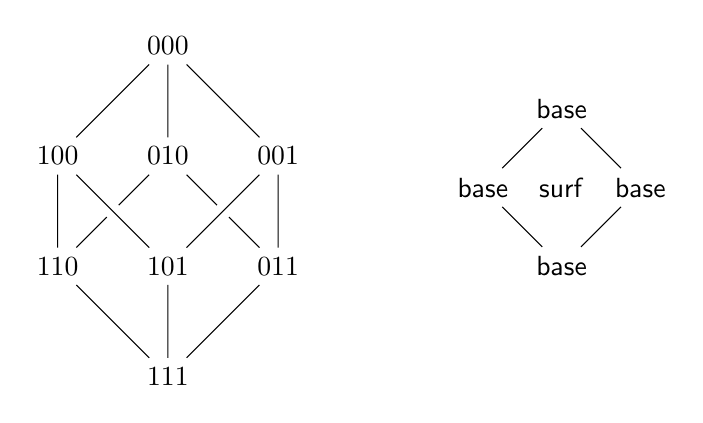
\begin{tikzpicture}
    \node (zzz) at (0,2.8) {$000$};
    \node (ozz) at (-1.4,1.4) {$100$};
    \node (zoz) at (0,1.4) {$010$};
    \node (ooz) at (-1.4,0) {$110$};
    \node (zzo) at (1.4,1.4) {$001$};
    \node (ozo) at (0,0) {$101$};
    \node (zoo) at (1.4,0) {$011$};
    \node (ooo) at (0,-1.4) {$111$};
    \draw (ooo) -- (ooz) -- (ozz) -- (zzz) -- (zoz) -- (zoo)
    (ozo) -- (ooo) -- (zoo) -- (zzo) -- (zzz)
    (ooz) -- (zoz);
    \draw[preaction={draw=white, -,line width=6pt}] (ozz) -- (ozo) -- (zzo);

    \begin{scope}[shift={(5,1)}]
      \node (zz) at (0,1) {\cset{base}};
      \node (zo) at (-1,0) {\cset{base}};
      \node (oz) at (1,0) {\cset{base}};
      \node (oo) at (0,-1) {\cset{base}};
      \node (filler) at (0,0) {\cset{surf}};
      \draw (zz) -- (zo) -- (oo) -- (oz) -- (zz);
    \end{scope}
  \end{tikzpicture}}\only<3>{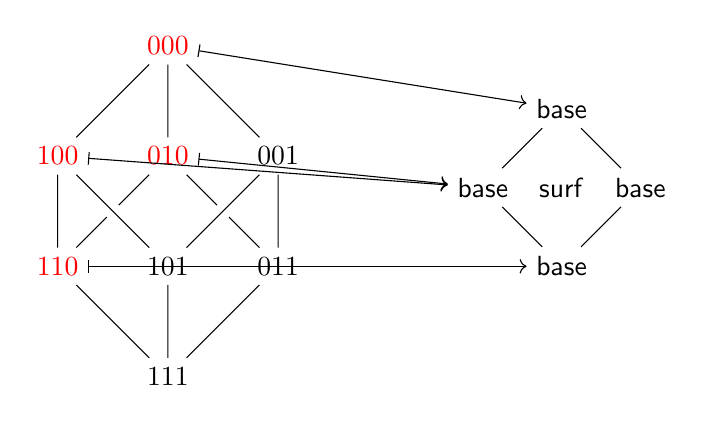
\begin{tikzpicture}
    \begin{scope}[color=red]
    \node (zzz) at (0,2.8) {$000$};
    \node (ozz) at (-1.4,1.4) {$100$};
    \node (zoz) at (0,1.4) {$010$};
    \node (ooz) at (-1.4,0) {$110$};
    \end{scope}
    \node (zzo) at (1.4,1.4) {$001$};
    \node (ozo) at (0,0) {$101$};
    \node (zoo) at (1.4,0) {$011$};
    \node (ooo) at (0,-1.4) {$111$};
    \draw (ooo) -- (ooz) -- (ozz) -- (zzz) -- (zoz) -- (zoo)
    (ozo) -- (ooo) -- (zoo) -- (zzo) -- (zzz)
    (ooz) -- (zoz);
    \draw[preaction={draw=white, -,line width=6pt}] (ozz) -- (ozo) -- (zzo);

    \begin{scope}[shift={(5,1)}]
      \node (zz) at (0,1) {\cset{base}};
      \node (zo) at (-1,0) {\cset{base}};
      \node (oz) at (1,0) {\cset{base}};
      \node (oo) at (0,-1) {\cset{base}};
      \node (filler) at (0,0) {\cset{surf}};
      \draw (zz) -- (zo) -- (oo) -- (oz) -- (zz);
    \end{scope}

    \draw[|->] (zzz) -- (zz);
    \draw[|->] (ozz) -- (zo);
    \draw[|->] (zoz) -- (zo);
    \draw[|->] (ooz) -- (oo);
  \end{tikzpicture}}\only<4>{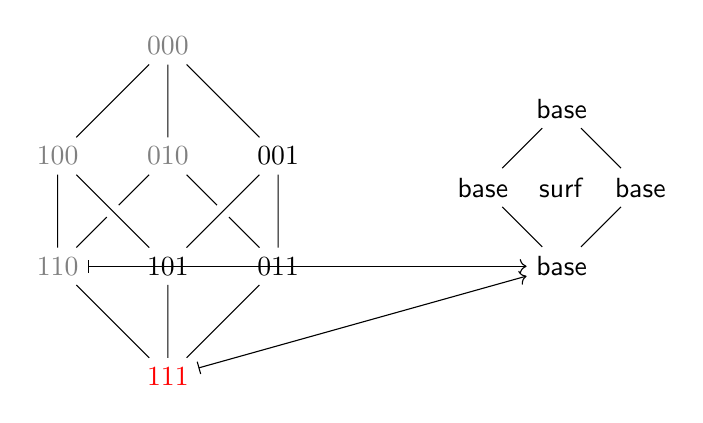
\begin{tikzpicture}
    \begin{scope}[color=gray]
    \node (zzz) at (0,2.8) {$000$};
    \node (ozz) at (-1.4,1.4) {$100$};
    \node (zoz) at (0,1.4) {$010$};
    \node (ooz) at (-1.4,0) {$110$};
    \end{scope}
    \node (zzo) at (1.4,1.4) {$001$};
    \node (ozo) at (0,0) {$101$};
    \node (zoo) at (1.4,0) {$011$};
    \node[color=red] (ooo) at (0,-1.4) {$111$};
    \draw (ooo) -- (ooz) -- (ozz) -- (zzz) -- (zoz) -- (zoo)
    (ozo) -- (ooo) -- (zoo) -- (zzo) -- (zzz)
    (ooz) -- (zoz);
    \draw[preaction={draw=white, -,line width=6pt}] (ozz) -- (ozo) -- (zzo);

    \begin{scope}[shift={(5,1)}]
      \node (zz) at (0,1) {\cset{base}};
      \node (zo) at (-1,0) {\cset{base}};
      \node (oz) at (1,0) {\cset{base}};
      \node (oo) at (0,-1) {\cset{base}};
      \node (filler) at (0,0) {\cset{surf}};
      \draw (zz) -- (zo) -- (oo) -- (oz) -- (zz);
    \end{scope}

    \draw[|->] (ooz) -- (oo);
    \draw[|->] (ooo) -- (oo);
  \end{tikzpicture}}\only<5>{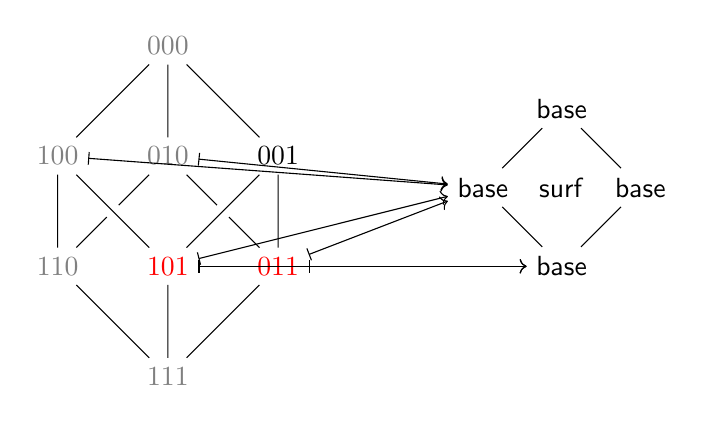
\begin{tikzpicture}
    \begin{scope}[color=gray]
      \node (zzz) at (0,2.8) {$000$};
      \node (ozz) at (-1.4,1.4) {$100$};
      \node (zoz) at (0,1.4) {$010$};
      \node (ooz) at (-1.4,0) {$110$};
    \end{scope}
    \node (zzo) at (1.4,1.4) {$001$};
    \node[color=red] (ozo) at (0,0) {$101$};
    \node[color=red] (zoo) at (1.4,0) {$011$};
    \node[color=gray] (ooo) at (0,-1.4) {$111$};
    \draw (ooo) -- (ooz) -- (ozz) -- (zzz) -- (zoz) -- (zoo)
    (ozo) -- (ooo) -- (zoo) -- (zzo) -- (zzz)
    (ooz) -- (zoz);
    \draw[preaction={draw=white, -,line width=6pt}] (ozz) -- (ozo) -- (zzo);

    \begin{scope}[shift={(5,1)}]
      \node (zz) at (0,1) {\cset{base}};
      \node (zo) at (-1,0) {\cset{base}};
      \node (oz) at (1,0) {\cset{base}};
      \node (oo) at (0,-1) {\cset{base}};
      \node (filler) at (0,0) {\cset{surf}};
      \draw (zz) -- (zo) -- (oo) -- (oz) -- (zz);
    \end{scope}

    \draw[|->] (ozz) -- (zo);
    \draw[|->] (zoz) -- (zo);
    \draw[|->] (ozo) -- (zo);
    \draw[|->] (ozo) -- (oo);
    \draw[|->] (zoo) -- (zo);
    \draw[|->] (zoo) -- (oo);
  \end{tikzpicture}}\only<6>{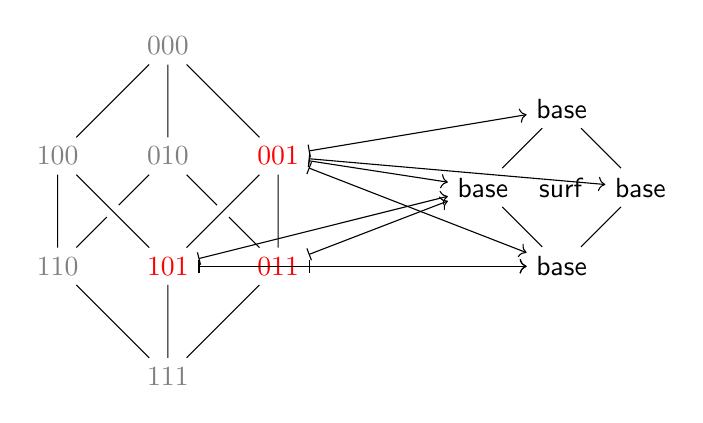
\begin{tikzpicture}
    \begin{scope}[color=gray]
      \node (zzz) at (0,2.8) {$000$};
      \node (ozz) at (-1.4,1.4) {$100$};
      \node (zoz) at (0,1.4) {$010$};
      \node (ooz) at (-1.4,0) {$110$};
    \end{scope}
    \node[color=red] (zzo) at (1.4,1.4) {$001$};
    \node[color=red] (ozo) at (0,0) {$101$};
    \node[color=red] (zoo) at (1.4,0) {$011$};
    \node[color=gray] (ooo) at (0,-1.4) {$111$};
    \draw (ooo) -- (ooz) -- (ozz) -- (zzz) -- (zoz) -- (zoo)
    (ozo) -- (ooo) -- (zoo) -- (zzo) -- (zzz)
    (ooz) -- (zoz);
    \draw[preaction={draw=white, -,line width=6pt}] (ozz) -- (ozo) -- (zzo);

    \begin{scope}[shift={(5,1)}]
      \node (zz) at (0,1) {\cset{base}};
      \node (zo) at (-1,0) {\cset{base}};
      \node (oz) at (1,0) {\cset{base}};
      \node (oo) at (0,-1) {\cset{base}};
      \node (filler) at (0,0) {\cset{surf}};
      \draw (zz) -- (zo) -- (oo) -- (oz) -- (zz);
    \end{scope}

    \draw[|->] (ozo) -- (zo);
    \draw[|->] (ozo) -- (oo);
    \draw[|->] (zoo) -- (zo);
    \draw[|->] (zoo) -- (oo);
    \draw[|->] (zzo) -- (zz);
    \draw[|->] (zzo) -- (zo);
    \draw[|->] (zzo) -- (oz);
    \draw[|->] (zzo) -- (oo);
  \end{tikzpicture}}



\end{center}

\end{frame}




% \begin{frame}
%   \frametitle{Example ppm}

% The following data represents the total ppm $\pint{5} \to \pint{1}$:
% \begin{align*}
% &00000\mapsto \{0,1\},00001\mapsto \{0,1\},00010\mapsto \{0,1\},00011\mapsto \{0,1\},\\
% &00100\mapsto \{0,1\},00101\mapsto \{0,1\},00110\mapsto \{0,1\},00111\mapsto \{0,1\},\\
% &01000\mapsto \{0,1\},01001\mapsto \{0,1\},01010\mapsto \{0,1\},01011\mapsto \{0,1\},\\
% &01100\mapsto \{0,1\},01101\mapsto \{0,1\},01110\mapsto \{0,1\},01111\mapsto \{0,1\},\\
% &10000\mapsto \{0,1\},10001\mapsto \{0,1\},10010\mapsto \{0,1\},10011\mapsto \{0,1\},\\
% &10100\mapsto \{0,1\},10101\mapsto \{0,1\},10110\mapsto \{0,1\},10111\mapsto \{0,1\},\\
% &11000\mapsto \{0,1\},11001\mapsto \{0,1\},11010\mapsto \{0,1\},11011\mapsto \{0,1\},\\
% &11100\mapsto \{0,1\},11101\mapsto \{0,1\},11110\mapsto \{0,1\},11111\mapsto \{0,1\}
% \end{align*}

% By calling $\Call{UnfoldPPM}{\Sigma}$ we compute all $7581$ poset maps.\\[.5em]

% We can get one poset map from a non-empty ppm in $\mathcal{O}(2^m 2^n)$,
% call this operation $\Call{FstPPM}{\Sigma}$. We can update $\Sigma$ at some $x$
% with $vs \subseteq \Sigma(x)$ in $\mathcal{O}(2^m 2^n)$, call this
% $\Call{UpdatePPM}{\Sigma,x,vs}$.

% \end{frame}


\begin{frame}
  \frametitle{Complexity of contortion search}

  When checking whether we can contort an $n$-cell into an $m$-dimensional
  boundary, we have to evaluate $\mathcal{O}(2mD_{m-1}^n)$ many contortions --
  bruteforce would require $\mathcal{O}(D_{m}^n)$.

  \vspace{1em} In many cases we have to check significantly fewer.

  \pause

  \begin{exampleblock}{}
  6-dim analogue of goal requires checking < 16.000 poset maps.
  % to ensure faces match. Runtime $< 2$s.
  \includegraphics[width=\textwidth]{img/6cube}

  Brute force: $D_6^2 = 7.828.354^2 = 61.283.126.349.316$ poset maps.

  \end{exampleblock}
\end{frame}

\begin{frame}
  \frametitle{Kan cubical sets}

  Crucial reasoning principle in Cubical Agda: $\mathsf{hcomp}$

  \begin{block}{}
    An $(n+1)$-dimensional open box is a collection of $2n + 1$ cells
    $[t_{1,\izero}, t_{1,\ione} , \ldots , t_{n,\izero}, t_{n,\ione}]u$ such that
    \begin{itemize}
    \item $\cont{t_{i,e}}{\dmap{n}{\izero}} = \cont{u}{\dmap{i}{e}}$ for all $1
      \leq i \leq n$ , $e \in \{\izero,\ione\}$
    \item $\cont{t_{i,e}}{\dmap{j}{e'}} = \cont{t_{j,e'}}{\dmap{i}{e}}$ for $1 \leq i < j \leq n$ and $e,e′ \in \{\izero,\ione\}$.
    \end{itemize}
  \end{block}

  \begin{block}{}
    A \mname{Kan cubical set} has for any open box $U$ a front side $\mathsf{Comp}\ U$.
    % $U = [( t_1, s_1 ), \ldots , (t_n , s_n)]u$ a cell $\comp{U}{}$ such that $[t_1,
    % s_1, \ldots , t_n , s_n , t, s]$ is a valid boundary:
  \end{block}

  \begin{exampleblock}{}
    \begin{columns}
      \begin{column}{.6\textwidth}
        \textbf{data} \cset{Paths} \textbf{where}
        \begin{itemize}
        \item $\cset{\star} : \cset{Paths}$
        \item $p,q,r : \star = \star$
          % \item $\cset{p} , \cset{q} , \cset{r} : \star = \star$
        \end{itemize}

        $p \pc q \mdef \mathsf{Comp}\ [\cont{\cset{\star}}{\smap{1}} , q ]p $
      \end{column}
      \begin{column}{.3\textwidth}
        \begin{tikzpicture}[scale=.5]
          \draw[->,>=stealth] (0,0) -- (3,0) node [midway,below, fill=none] {$p$};
          \draw[->,dotted,>=stealth] (0,3) -- (3,3) node [midway,above, fill=none] {$p \pc q$};
          \draw[->,>=stealth] (0,0) -- (0,3) node [midway,left,  fill=none] {$\cont{\star}{\smap{1}}$};
          \draw[->,>=stealth] (3,0) -- (3,3) node [midway,right, fill=none] {$q$};
        \end{tikzpicture}
      \end{column}
    \end{columns}

\end{exampleblock}

\end{frame}


\begin{frame}
  \frametitle{Finding open boxes as a constraint satisfaction problem}

  % Constraint satisfaction problems (CSP) express a large class of algorithmic
  % problems.

  % Construct an open box with $T$ on front by solving this CSP:

  \begin{columns}
    \begin{column}{.6\textwidth}
      \begin{block}{}
        \mname{Problem \textbf{KanCubicalCell}}: given a boundary $T$, find an open
        cube $U$ with front $T$.
      \end{block}
    \end{column}
    \begin{column}{.4\textwidth}
      \hcompcubesmall{}{}{}{}{X_{1,\izero}}{X_{2,\izero}}{X_{1,\ione}}{X_{2,\ione}}{X_\text{B}}
    \end{column}
  \end{columns}

  \pause

  \begin{block}{}
    \begin{itemize}
    \item  Variables $X_{\text{B}}$ and $X_{i,\izero}$, $X_{i,\ione}$ for $1 \leq
      i \leq n$
    \item Domains 
      \begin{itemize}
      \item $D_{\text{B}} = \{ \cont{p}{\Sigma} \mid p \in \Gamma \}$
      \item $D_{i,e} = \{ \cont{p}{\Sigma} \mid p \in \Gamma,
      \cont{\cont{p}{\Sigma}}{\dmap{n}{\ione}} = T_{i,e} \}$
      \end{itemize}
    \item Constraints
    \begin{itemize}
    \item $\cont{X_{i,e}}{\dmap{n}{\izero}} = \cont{X_{\text{B}}}{\dmap{i}{e}}$ for all $1
      \leq i \leq n$ , $e \in \{\izero,\ione\}$
    \item $\cont{X_{i,e}}{\dmap{j}{e'}} = \cont{X_{j,e'}}{\dmap{i}{e}}$ for $1 \leq i < j \leq n$, $e,e′ \in \{\izero,\ione\}$.
    \end{itemize}
  \end{itemize}
  \end{block}


  % \begin{columns}
  %   \begin{column}{.6\textwidth}
  %     \begin{itemize}
  %     \item Variables $X_{\text{B}}$ and $X_{k,\izero}$,
  %       $X_{k,\ione}$ for $1 \leq k \leq n$ stand for the side and back
  %       faces of the cube.
  %     \item Domains are all $\cont{p}{\Sigma}$ for $p\in \Gamma$ matching the goal.
  %       $D_{B}$ are all shapes, $D_{1, 0}, D_{1, 1} , D_{2,0} , D_{2,1}$ restricted to match goal
  %       boundary

  %       TODO
  %     \item Contraints are that all boundaries of the sides and back need to
  %       match: TODO
  %     \end{itemize}
  %   \end{column}
  %   \begin{column}{.4\textwidth}
  %     \hcompcubesmall{}{}{}{}{X_{1,\izero}}{X_{2,\izero}}{X_{1,\ione}}{X_{2,\ione}}{X_\text{B}}

  %   \end{column}
  % \end{columns}


  % \begin{itemize}
  % \item Variables $X_{B}$ and $X_{i_k,\izero}$, $X_{i_k,\ione}$ for $1 \leq k
  %   \leq n$.
  % \item Domains $D_{B} = S$ and $D_{i_k,e} = \{ t \in S :
  %   \boundary{t}{n}{\ione} = \boundary{\Phi}{k}{e} \}$ for $1 \leq k \leq n$,
  %   $e \in \{\izero, \ione\}$.
  % \item Constraints
  %   \begin{itemize}
  %   \item $\boundary{X_{i_k,e}}{n}{\izero} = \boundary{X_B}{k}{e}$ for $k = 1,
  %     ... , n$, $e \in \{\izero, \ione\}$.
  %   \item $\boundary{X_{i_k,e}}{k+e}{e'} = \boundary{X_{i_l,e'}}{l-e'}{e} $
  %     for $1 \leq k < l \leq n$, $e, e' \in \{\izero, \ione\}$.
  %   \end{itemize}
  % \end{itemize}

\end{frame}



\begin{frame}
  \frametitle{Simple Kan composition}

  \begin{exampleblock}{}
    \textbf{data} \cset{Paths} \textbf{where}
    \begin{itemize}
    \item $\cset{\star} : \cset{Paths}$
    \item $p,q : \star = \star$
      % \item $\cset{p} , \cset{q} , \cset{r} : \star = \star$
    \end{itemize}
  \end{exampleblock}

  \textbf{Goal:} $\mlist{p,q,p,q}$

  \begin{columns}
    \begin{column}{.45\textwidth}
      \only<1>{\hcompcubesmall{p}{p}{q}{q}{X_{1,\izero}}{X_{2,\izero}}{X_{1,\ione}}{X_{2,\ione}}{X_\text{B}}}\only<2>{\hcompcubesmall{p}{p}{q}{q}{p\ i}{p\ i}{q \wedge}{q \wedge}{p \vee}}
    \end{column}
    \begin{column}{.6\textwidth}
      \only<1>{
      $D_{1,0} = \{ \cont{{p}}{\substfour{0}{0,1}{0}{1}} \}$

      $D_{1,1} = \{ \cont{{q}}{\substfour{0}{0,1}{0}{1}} \}$

      $D_{1,0} = \{ \cont{{p}}{\substfour{0}{0,1}{0}{1}} \}$

      $D_{1,1} = \{ \cont{{q}}{\substfour{0}{0,1}{0}{1}} \}$

      $D_{B} = \{ \cont{\cset{\star}}{\substfour{()}{()}{()}{()}} ,
      \cont{{p}}{\substfour{0,1}{0,1}{0,1}{0,1}},
      \cont{{q}}{\substfour{0,1}{0,1}{0,1}{0,1}}
      \}$
      }\only<2>{
      $D_{1,0} = \{ \cont{{p}}{\substfour{0}{1}{0}{1}} \}$

      $D_{1,1} = \{ \cont{{q}}{\substfour{0}{0}{0}{1}} \}$

      $D_{1,0} = \{ \cont{{p}}{\substfour{0}{1}{0}{1}} \}$

      $D_{1,1} = \{ \cont{{q}}{\substfour{0}{0}{0}{1}} \}$

      $D_{B} = \{ \cont{{p}}{\substfour{0}{1}{1}{1}} \}$
      }
    \end{column}
  \end{columns}


% \only<2>{
%   \begin{center}
%     \hcompcube
%     {p}{q}
%     {p}{q}
%     {p\ i}{q \wedge}
%     {p\ i}{q \wedge}
%     {p \vee}
%     % {\cont{p}{\appfstsubst}}{\cont{q}{\andsubst}}
%     % {\cont{p}{\appfstsubst}}{\cont{q}{\andsubst}}
%     % {\cont{p}{\orsubst}}
%   \end{center}
% }
\end{frame}



\begin{frame}
  \frametitle{Associativity of path composition}

  \begin{exampleblock}{}
    \textbf{data} \cset{Paths} \textbf{where}
    \begin{itemize}
    \item $\cset{\star} : \cset{Paths}$
    \item $p,q,r : \star = \star$
    % \item $\cset{p} , \cset{q} , \cset{r} : \star = \star$
    \end{itemize}
  \end{exampleblock}

  \textbf{Goal:} $(p \pc q) \pc r = p \pc (q \pc r) \ \ \rightsquigarrow \ \ \mlist{(p \pc q) \pc r , p \pc (q \pc r) ,
    \cont{\star}{\smap{1}} , \cont{\star}{\smap{1}}}$ % (``$(p \pc q) \pc r = p \pc (q \pc r)$'')
  \begin{center}
    \only<1>{
      \hcompcube
        {(p \pc q) \pc r}{p \pc (q \pc r)}
        {\cont{\star}{\smap{1}}}{\cont{\star}{\smap{1}}}
        {}{}{}{}
        {}
  }\only<2>{
    \hcompcube
      {(p \pc q) \pc r}{p \pc (q \pc r)}
      {\cont{\star}{\smap{1}}}{\cont{\star}{\smap{1}}}
      {\pcfill{p \pc q}{r}}{\pcfill{p}{q \pc r}}
      {}{}
      {}
  }\only<3>{
    \hcompcube
    {(p \pc q) \pc r}{p \pc (q \pc r)}
    {\cont{\star}{\smap{1}}}{\cont{\star}{\smap{1}}}
    {\pcfill{p \pc q}{r}}{\pcfill{p}{q \pc r}}
    {\cont{\star}{\smap{2}}}{?}
    {?}
  }
  \end{center}

  \vspace{-1em}
  \only<2>{\begin{idea}
    Unfold Kan compositions of goal boundary
  \end{idea}}\onslide<3>{\begin{idea}
    Fill sides with contortions if possible
  \end{idea}}


\end{frame}

\begin{frame}
  \frametitle{Filling the open sides}

  \begin{columns}
    \begin{column}{.5\textwidth}
      Filler for the back:\\[1em]
  \begin{tikzpicture}[scale=.85]
    \draw[->,>=stealth] (0,0) -- (4,0) node [midway,below, fill=none] {\ensuremath{p \pc q}};
    \draw[->,>=stealth] (0,4) -- (4,4) node [midway,above, fill=none] {\ensuremath{p}};
    \draw[->,>=stealth] (0,0) -- (0,4) node [midway,left=.2cm, fill=none] {\ensuremath{\cont{\star}{\smap{1}}}};
    \draw[->,dashed,>=stealth] (4,0) -- (4,4) node [midway,right=.2cm,fill=none] {\only<3->{\ensuremath{\inv{q}}}};

    \draw[->,>=stealth] (1.2,1.2) -- (2.8,1.2);
    \draw[->,>=stealth] (1.2,1.2) -- (1.2,2.8);
    \draw[->,>=stealth] (2.8,1.2) -- (2.8,2.8);
    \draw[->,>=stealth] (1.2,2.8) -- (2.8,2.8);

    \draw[->,>=stealth] (1.2,1.2) -- (0,0);
    \draw[->,>=stealth] (2.8,1.2) -- (4,0);
    \draw[->,>=stealth] (2.8,2.8) -- (4,4);
    \draw[->,>=stealth] (1.2,2.8) -- (0,4);

    \node at (2, .6)  {\ensuremath{\pcfill{p}{q}}};
    \node at (2, 3.4) {\ensuremath{\only<2->{\cont{p}{\appfstsubst}}}};
    \node at (.6, 2)  {\ensuremath{\only<2->{\cont{\star}{\smap{2}}}}};
    \node at (3.4, 2) {\ensuremath{}};
    \node at (2, 2)  {\ensuremath{\only<2->{\cont{p}{\appsndsubst}}}};
  \end{tikzpicture}
      % \hcompcube
      % {p \pc q}{p}
      % {\cont{\star}{\smap{1}}}{\inv{q}}
      % {\pcfill{p}{q}}{\cont{p}{\appfstsubst}}
      % {\cont{\star}{\smap{2}}}{\invfill{q}}
      % {\cont{p}{\appsndsubst}}
    \end{column}
    \begin{column}{.5\textwidth}
      \onslide<3->{
        Filler for the right side:\\[1em]
        \hcompcube
        {r}{q \pc r}
        {\inv{q}}{\cont{\star}{\smap{1}}}
        {\Theta}{\pcfill{q}{r}}
        {}{\cont{r}{\appsndsubst}}
        {\cont{q}{\appsndsubst}}

        % \begin{center}
        %   \includegraphics[scale=.4]{img/assoc}
        % \end{center}
      }
    \end{column}
  \end{columns}

  \onslide<3->{
  \begin{idea}{}
    % If goal boundary unspecified, fill with Kan composition if necessary
    Open faces can be filled with Kan fillers
    % Fill sides that have open boundary with Kan filler (if necessary)
  \end{idea}
  }
\end{frame}



\begin{frame}
  \frametitle{Kan composition algorithm}

  Given goal $T$, construct a nested Kan composition as follows:

  \begin{itemize}
  \item Solve CSP for open box with front boundary $T$
    \begin{itemize}
    \item Unfold Kan compositions if possible
    \item Fill as many sides with contortions as possible
    \item If not all sides can be filled, use Kan fillers for open faces
    \end{itemize}
  \item Call composition solver on open sides of the cube
  \end{itemize}

  Complete calculus. CSPs stay small, not much memory needed.
\end{frame}


\begin{frame}
  \frametitle{Proving Eckmann-Hilton}

  \begin{exampleblock}{}
  \textbf{data} \cset{EckmannHilton} \textbf{where}
  \begin{itemize}
  \item $\cset{\star} : \cset{EckmannHilton}$
  \item $p,q : \mathsf{Path}\ (\mathsf{Path}\
    \cset{EckmannHilton}\ \cset{\star}\ \cset{\star})\ \mathsf{refl}\ \mathsf{refl}$
  \end{itemize}
\end{exampleblock}

\textbf{Goal:} $p \pc q = q \pc p \quad \rightsquigarrow$

  $\qquad\quad [
  \mathsf{Comp}\ [\cont{\cset{\star}}{\smap{1}} , q ,
  \cont{\cset{\star}}{\smap{1}} , \cont{\cset{\star}}{\smap{1}} ]p,
  \mathsf{Comp}\ [\cont{\cset{\star}}{\smap{1}} , p ,
  \cont{\cset{\star}}{\smap{1}} , \cont{\cset{\star}}{\smap{1}} ]q,$

  $\qquad\quad \  \cont{\cset{\star}}{\smap{2}},\cont{\cset{\star}}{\smap{2}},
  \cont{\cset{\star}}{\smap{2}},\cont{\cset{\star}}{\smap{2}}]$\\[1em]
  \pause
  Prove this in two steps:
  \begin{itemize}
  \item Fill the cube 
    $\mlist{p,p,q,q,\cont{\star}{\smap{2}} , \cont{\star}{\smap{2}}}$
  % \item Show $t : \mlist{p,q,p,q}$ gives rise to $t' : \mlist{p \pc q , p \pc q , \cont{\star}{\smap{1}} , \cont{\star}{\smap{1}}}$

  %   \filledsquare{p}{q}{p}{q}{t} $\qquad$
  %   \filledsquare{p \pc q}{p \pc q}
  %   {\cont{\star}{\smap{1}}}
  %   {\cont{\star}{\smap{1}}}
  %   {t'}

  \item Show $t : \mlist{p,s,r,q}$ gives rise to $t' : \mlist{p \pc q , r \pc s , \cont{\star}{\smap{1}} , \cont{\star}{\smap{1}}}$

    \filledsquare{p}{s}{r}{q}{t} $\qquad$
    \filledsquare{p \pc q}{r \pc s}
    {\cont{\star}{\smap{1}}}
    {\cont{\star}{\smap{1}}}
    {t'}

    \only<2>{\begin{textblock}{10}(6,13)
      $\mapsto$
    \end{textblock}}
  \end{itemize}
\end{frame}


\begin{frame}
  \frametitle{Conclusions}

  \begin{itemize}
  \item The problem of finding Kan cubical cells generalises word problems for various algebraic structures,
    satisfiability, ...

    $\to$ derivation \emph{spaces} instead of trees
  \item Desired takeaways:
    \begin{itemize}
    \item \emph{Practical}: develop a tactic for automatic proof search. Can we derive new proofs?
    \item \emph{Foundational}: even in weak model, can we discard most coherences
      automatically? Have to leave the garden eden of decidability...
      % we don't want to die virtuously
    \end{itemize}
  % \item Make tactic part of Cubical Agda.
    % \begin{itemize}
    % \item Use macro to extract proof goal, pass to Haskell solver with
    %   \texttt{execTC}, macro parses string into internal \texttt{Term}.
    %   % Pro: fast and already implemented
    %   % Con: introduces dependencies, Read not yet implemented
    % \item Rebuild solver in Agda, make part of Cubical library.
    %   % Pro: no dependencies, doesn't require fixes in Agda, should be more stable
    %   % Con: slower, have to reimplement everything in dependent type theory
    % \end{itemize}
  % \item Allow for free faces in solver % DO I WANT TO TALK ABOUT SOMETHING SO TECHNICAL?
  % \item Improve search for ``admissible rules'': Inverse paths, fillers
  % \item Formalize proofs which so far have been out of reach: Pentagon of smash
  %   product, ..., ?
  \end{itemize}

  \onslide<2>{
    \begin{block}{}
      \center
    Thank you for your attention!
  \end{block}
  }
\end{frame}


% % \begin{frame}
% %   \frametitle{References}
% %   \bibliography{bibliography}
% % \end{frame}

\appendix
\backupbegin

\begin{frame}
  \frametitle{Demos}
  \begin{center}
    \includegraphics[scale=.3]{img/assoc}
    \includegraphics[scale=.5]{img/ehsquare}
    \includegraphics[scale=.5]{img/squareswitch}
  \end{center}
\end{frame}


\begin{frame}
  \frametitle{In summary}

  \begin{center}
    $n$-tuples of terms in $m$-element bounded distributive lattice

    $\simeq$

    monotone maps $\{ 0<1 \}^m \to \{ 0<1 \}^n$
  \end{center}
\end{frame}


\begin{frame}
  \frametitle{Formal definitions?}

  % We have numerous flavors of cubes presented in numerous ways. Nominal sets
  % e.g., but also cartesian, De Morgan, disjunctive, \textbf{Dedekind}...

  % Dedekind cubes have a nice geometric presentation which makes it apt for proof
  % search.


  $\dedekind$ is the full subcategory of the category
  of posets and monotone maps with objects $\pint{n}$ for $n \geq 0$, where $\pint{}
  = \{ 0<1 \}$.\\[.5em]

  % Therefore morphisms in $\dedekind$ are of
  % the form $\pint{m} \to \pint{n}$.

  All morphisms in $\dedekind$ are of the form $\pint{m} \to \pint{n}$, e.g.:
  \begin{align*}
    \smap{i} &: \pint{n} \to \pint{n-1}, (e_1 \ldots e_n) \mapsto (e_1 \ldots e_{i-1} e_{i+1} \ldots e_n) \text{ for } 1 \leq i \leq n\\
    \dmap{i}{e} &: \pint{n-1} \to \pint{n}, 
                (e_1 \ldots e_{n-1}) \mapsto (e_1 \ldots e_{i-1} e e_{i+1} \ldots e_{n-1}) \\&\qquad\qquad\qquad\qquad\qquad\qquad\qquad\qquad
    \text{ for } 1 \leq i \leq n, e \in \{0,1\}
  \end{align*}

  Cubical sets are objects of $\psh{\dedekind}$.\\[.5em]

  % For a cubical set $X$ write $X_n \mdef X(\pint{n})$ for its $n$-cells, $\smap{i} \mdef X(s^i) :
  % X_{n-1} \to X_n$ and $\dmap{i}{e} \mdef X(d^{(i,e)}) : X_n \to X_{n-1}$.\\[.5em]

  Given an $n$-cell $p$ of a cubical set $X$ and a poset map $\sigma :
  \pint{m} \to \pint{n}$, call $\cont{p}{\sigma} \mdef X(\sigma)(p)$ an
  $m$-contortion of $p$.\\[1em]

  TODO DO WE WANT BELOW NOTION ON BOUNDARY?
  Its boundary is
  $\boundary{p} \mdef [\cont{p}{d^{(1,\izero)}} , \cont{p}{d^{(1,\ione)}} , \ldots
  \cont{p}{d^{(n,\izero)}} , \cont{p}{d^{(n,\ione)}}]$
\end{frame}



\begin{frame}
  \frametitle{Higher inductive types}

  We describe cubical sets by giving the generating cells:
  
  \begin{block}{}
    % A \mname{boundary} is a list of $2\cdot n$ many $(n-1)$-dimensional cells
    % $(t_1, s_1), \ldots , (t_n , s_n)$ (whose boundaries match).\\[1em]
  A \mname{context} $\Gamma$ is a list of declarations $\mlist{p_1 : T_1 , \ldots , p_k
  : T_k}$. The cubical set $X$ generated by $\Gamma$ has non-degenerate cells
  $p_i$ with $\boundary{p_i} = T_i$ valid boundaries and all necessary contortions.
  \end{block}

  \vspace{1em}
  \begin{columns}
    \begin{column}{.6\textwidth}
      \textbf{Interval:}
      
    $\mlist{ \cset{zero} : \mlist{} , \cset{one} : \mlist{} , \cset{seg} : \mlist{
          \cont{\cset{zero}}{}, \cont{\cset{one}}{} }}$
    \end{column}
    \begin{column}{.4\textwidth}
      $\cset{zero}\xrightarrow{\cset{seg}}\cset{one}$
    \end{column}
  \end{columns}
  % \vspace{1em}
      \begin{columns}
        \begin{column}{.6\textwidth}
          \textbf{Sphere:}
          $\mlist{ \cset{a} : \mlist{} , \cset{p} : \mlist{ \cont{\cset{a}}{\oneconst}
              , \cont{\cset{a}}{\oneconst} , \cont{\cset{a}}{\oneconst},
              \cont{\cset{a}}{\oneconst} }}$
        \end{column}
        \begin{column}{.4\textwidth}
          \filledsquare{\cont{\cset{a}}{\oneconst}}{\cont{\cset{a}}{\oneconst}}{\cont{\cset{a}}{\oneconst}}{\cont{\cset{a}}{\oneconst}}{\cset{p}}
        \end{column}
      \end{columns}


      \begin{columns}
        \begin{column}{.6\textwidth}
          \textbf{Triangle}
      $\mlist{ \cset{x} : \mlist{} , \cset{y} : \mlist{} , \cset{z} : \mlist{} ,
        \cset{p} : \mlist{ \cset{x}, \cset{y}  } ,
        , \cset{q} : \mlist{ \cset{y}, \cset{z} }
        , \cset{r} : \mlist{ \cset{x}, \cset{z} }
        , \cset{\phi} : \mlist{ \cset{p} , \cset{r} ,
          \cont{\cset{x}}{\oneconst}, \cset{q} }
      }$
    \end{column}
    \begin{column}{.4\textwidth}
      % \filledsquare{\cont{\cset{a}}{\oneconst}}{\cont{\cset{a}}{\oneconst}}{\cont{\cset{a}}{\oneconst}}{\cont{\cset{a}}{\oneconst}}{\cset{p}}
    \end{column}
  \end{columns}
\end{frame}



\begin{frame}
  \frametitle{Boundaries as proof goals}

  \begin{exampleblock}{}
    \textbf{Second loopspace:}
    $\mlist{ \cset{a} : \mlist{} , \cset{p} : \mlist{ \cont{\cset{a}}{\oneconst}
        , \cont{\cset{a}}{\oneconst} , \cont{\cset{a}}{\oneconst},
        \cont{\cset{a}}{\oneconst} }}$
  \end{exampleblock}

  Goal: Find $\sigma : \pint{3} \to \pint{2}$ such that
  $\cont{p}{\sigma}$ has this boundary:


  $$\mlist{ \cont{\cset{p}}{\substfour{00}{01}{01}{11}} ,
    \cont{\cset{a}}{\smap{2}} , \cont{\cset{a}}{\smap{2}} ,
    \cont{\cset{a}}{\smap{2}} , \cont{\cset{a}}{\smap{2}} , \cont{\cset{a}}{\smap{2}}}$$
      \textcolor{gray}{ In Cubical:\vspace{-1em}
  \begin{align*}
    \mathsf{PathP} (\lambda i \to \mathsf{PathP} &(\lambda j \to  \mathsf{Path} \ (\cset{p} \ (i \wedge
                                                       j) \ (i \vee j))\ \cset{a})\\
                                                     &(\lambda j \to \cset{a}) (\lambda j \to \cset{a}))
                                                     (\lambda i j \to \cset{a}) (\lambda i j \to \cset{a})
  \end{align*}
}

There are $D_3^2 = 20^2 = 400$ poset maps $\pint{3} \to \pint{2}$ which could fit. \\[.5em]

In general: $D_m^n$ many morphisms $\pint{m} \to \pint{n}$, where $D_m$
is the $m$-th Dedekind number ($D_5 = 7581, D_6 = 7828354 , ... ,D_9 = ?$). \\[.5em]

$\to$ Need efficient representation for collections of poset maps.
\end{frame}


\begin{frame}
  \frametitle{Potential contortions}

  ppms give us some information   of all poset maps in them:

  \begin{columns}
    \begin{column}{.4\textwidth}
      $\cont{\cset{seg}}{\substfourlarge{\{0\}}{\{0, 1\}}{\{0, 1\}}{\{1\}}}$
    \end{column}
    \begin{column}{.6\textwidth}

      \begin{tikzpicture}[scale=1.3]
        % \node (zz) at (0,1) {\textcolor{gray}{00} $\mapsto \{x\}$};
        % \node (zo) at (-1,0) {\textcolor{gray}{01} $\mapsto \{x , y\}$};
        % \node (oz) at (1,0) {\textcolor{gray}{10} $\mapsto \{x , y\}$};
        % \node (oo) at (0,-1) {\textcolor{gray}{11} $\mapsto \{y\}$};
        \node (zz) at (0,1) {\textcolor{gray}{00}};
        \node (zo) at (-1,0) {\textcolor{gray}{01}};
        \node (oz) at (1,0) {\textcolor{gray}{10}};
        \node (oo) at (0,-1) {\textcolor{gray}{11}};
        \draw (zz) -- (zo) -- (oo) -- (oz) -- (zz);
        % \end{tikzpicture}
        % \begin{tikzpicture}[scale=1]
          \node (z) at (2.6,.7) {\cset{zero}};
          \node (o) at (2.6,-.7) {\cset{one}};
          \draw (z) -- (o) node[midway,right] {\cset{seg}};

          \draw[|->] (zz) -- (z);
          \draw[|->] (zo) -- (z);
          \draw[|->] (zo) -- (o);
          \draw[|->] (oz) -- (o);
          \draw[|->] (oz) -- (z);
          \draw[|->] (oo) -- (o);
      \end{tikzpicture}
    \end{column}
  \end{columns}

  \vspace{1em}
  Thereby we have captured these four squares:

  \begin{columns}
    \begin{column}{.25\textwidth}
      \filledsquare{\cset{seg}}{\cset{seg}}{\phantom{\cset{seg}}}{\phantom{\cset{seg}}}{\substfour{0}{0}{1}{1}}
    \end{column}
    \begin{column}{.25\textwidth}
      \filledsquare{\phantom{\cset{seg}}}{\phantom{\cset{seg}}}{\cset{seg}}{\cset{seg}}{\substfour{0}{1}{0}{1}}
    \end{column}
    \begin{column}{.25\textwidth}
      \filledsquare{\cset{seg}}{\phantom{\cset{seg}}}{\cset{seg}}{\phantom{\cset{seg}}}{\substfour{0}{1}{1}{1}}
    \end{column}
    \begin{column}{.25\textwidth}
      \filledsquare{\phantom{\cset{seg}}}{\cset{seg}}{\phantom{\cset{seg}}}{\cset{seg}}{\substfour{0}{0}{0}{1}}
    \end{column}
  \end{columns}

  % TODO HIGHLIGHT WHICH BOUNDARY IS FIXED
\end{frame}


\begin{frame}
  \frametitle{Triangle slide}

  \begin{exampleblock}{}
    \textbf{Triangle:}

    $\mlist{ \cset{x} : \mlist{} , \cset{y} : \mlist{} , \cset{z} : \mlist{} ,
      \cset{p} : \mlist{ \cset{x}, \cset{y}  } ,
      , \cset{q} : \mlist{ \cset{y}, \cset{z} }
      , \cset{r} : \mlist{ \cset{x}, \cset{z} }
      , \cset{\phi} : \mlist{ \cset{p} , \cset{r} ,
        \cont{\cset{x}}{\oneconst}, \cset{q} }
    }$
  \end{exampleblock}

  Goal: Find a cell with boundary $\mlist{\cset{r} , \cset{q} , \cset{p} , \cont{\cset{z}}{\smap{1}}}$

  \begin{columns}
    \begin{column}{.45\textwidth}
      \hcompcubesmall{\cset{r}}{\cset{p}}{\cset{q}}{\cont{\cset{z}}{\smap{1}}}{X_{1,\izero}}{X_{2,\izero}}{X_{1,\ione}}{X_{2,\ione}}{X_\text{B}}
    \end{column}
    \begin{column}{.55\textwidth}
      $D_{1,0} = \{ \cont{\cset{r}}{\small
      \arraycolsep=.4pt\def\arraystretch{1}
      \begin{array}{lcl}
      00 & \mapsto & \{0\} \\
      01 & \mapsto & \{0,1\} \\
      10 & \mapsto & \{0\} \\
      11 & \mapsto & \{1\}
      \end{array}}
      \}$

      $...$\\[1em]

      $D_{B} \{ ... , \cont{\phi}{\small
      \arraycolsep=.4pt\def\arraystretch{1}
      \begin{array}{lcl}
        00 & \mapsto & \{00 , 01 , 10 , 11\} \\
        01 & \mapsto & \{00 , 01 , 10 , 11\} \\
        10 & \mapsto & \{00 , 01 , 10 , 11\} \\
        11 & \mapsto & \{00 , 01 , 10 , 11\}
      \end{array}} \}$
    \end{column}
  \end{columns}
\end{frame}


\begin{frame}
  \frametitle{Vertex constraint}

  \begin{columns}
    \begin{column}{.45\textwidth}
      \hcompcubesmall{\cset{r}}{\cset{p}}{\cset{q}}{\cont{\cset{z}}{\smap{1}}}{X_{1,\izero}}{X_{2,\izero}}{X_{1,\ione}}{X_{2,\ione}}{X_\text{B}}
      % \dimcube{i}{j}{k}

    \end{column}
    \begin{column}{.55\textwidth}
      $D_{1,0} = \{ \cont{\cset{r}}{\small
      \arraycolsep=.4pt\def\arraystretch{1}
      \begin{array}{lcl}
        00 & \mapsto & \textcolor{blue}{\{0\}} \\
        01 & \mapsto & \{0,1\} \\
        10 & \mapsto & \{0\} \\
        11 & \mapsto & \{1\}
      \end{array}} \}$

      $...$\\[1em]

      $D_{B} = \{ ... , \cont{\phi}{\small
      \arraycolsep=.4pt\def\arraystretch{1}
      \begin{array}{lcl}
        00 & \mapsto & \{\textcolor{blue}{00} , \cancel{\textcolor{red}{01}} , \textcolor{blue}{10} , \cancel{\textcolor{red}{11}}\} \\
        01 & \mapsto & \{00 , 01 , 10 , 11\} \\
        10 & \mapsto & \{00 , 01 , 10 , 11\} \\
        11 & \mapsto & \{00 , 01 , 10 , 11\}
      \end{array}} \}$

    \end{column}
  \end{columns}

  \begin{columns}
    \begin{column}{.4\textwidth}
      \begin{center}
        
      \begin{tikzpicture}[scale=.8]
        \node (zz) at (0,1) {\textcolor{gray}{00}};
        \node (zo) at (-1,0) {\textcolor{gray}{01}};
        \node (oz) at (1,0) {\textcolor{gray}{10}};
        \node (oo) at (0,-1) {\textcolor{gray}{11}};
        \draw (zz) -- (zo) -- (oo) -- (oz) -- (zz);
        % \end{tikzpicture}
        % \begin{tikzpicture}[scale=1]
          \node (z) at (2.6,.7) {$\cset{x}$};
          \node (o) at (2.6,-.7) {$\cset{z}$};
          \draw (z) -- (o) node[midway,right] {$\cset{r}$};

          \draw[|->] (zz) -- (z);
          % \draw[|->] (zo) -- (z);
          % \draw[|->] (zo) -- (o);
          % \draw[|->] (oz) -- (o);
          % \draw[|->] (oz) -- (z);
          % \draw[|->] (oo) -- (o);
      \end{tikzpicture}
    \end{center}
    \end{column}

    \begin{column}{.6\textwidth}
      \begin{center}
      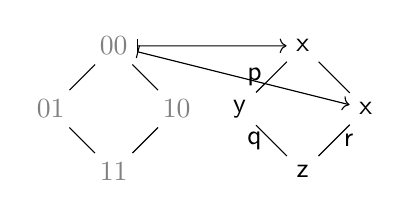
\begin{tikzpicture}[scale=.8]
        \node (zz) at (0,1) {\textcolor{gray}{00}}; \node (zo) at (-1,0)
        {\textcolor{gray}{01}}; \node (oz) at (1,0) {\textcolor{gray}{10}};
        \node (oo) at (0,-1) {\textcolor{gray}{11}}; \draw (zz) -- (zo) --
        (oo) -- (oz) -- (zz);

        \node (zz2) at (3,1) {$\cset{x}$};
        \node (zo2) at (2,0) {$\cset{y}$};
        \node (oz2) at (4,0) {$\cset{x}$};
        \node (oo2) at (3,-1) {$\cset{z}$};

        \draw (zz2) -- (zo2) node[midway,left] {$\cset{p}$};
        \draw (zz2) -- (oz2) node[midway,right] {};
        \draw (oz2) -- (oo2) node[midway,right] {$\cset{r}$};
        \draw (zo2) -- (oo2) node[midway,left] {$\cset{q}$};

        % TODO DRAW EDGE LABELS

        \draw[|->] (zz) -- (zz2);
        \draw[|->] (zz) -- (oz2);
      \end{tikzpicture}
    \end{center}
    \end{column}

    \end{columns}


\end{frame}

\begin{frame}
  \frametitle{Edge constraint}

  \begin{columns}
    \begin{column}{.45\textwidth}
      \hcompcubesmall{\cset{r}}{\cset{p}}{\cset{q}}{\cont{\cset{z}}{\smap{1}}}{X_{1,0}}{X_{2,\izero}}{X_{1,\ione}}{X_{2,\ione}}{X_\text{B}}
      % \dimcube{i}{j}{k}

    \end{column}
    \begin{column}{.55\textwidth}
      $...$\\[1em]

      $D_{1,0} = \{ \cont{\cset{r}}{\small
      \arraycolsep=.4pt\def\arraystretch{1}
      \begin{array}{lcl}
        00 & \mapsto & \{0\} \\
        01 & \mapsto & \textcolor{blue}{\{0\}} \\
        10 & \mapsto & \{0\} \\
        11 & \mapsto & \textcolor{blue}{\{1\}}
      \end{array}} \}$

      \ 

      $D_{2,1} = \{ ... , \cont{\phi}{\small
      \arraycolsep=.4pt\def\arraystretch{1}
      \begin{array}{lcl}
        00 & \mapsto & \{\cancel{\textcolor{red}{00}} , \textcolor{blue}{10} \} \\
        01 & \mapsto & \only<1>{\{00 , 01 , 10 , 11\}} \only<2>{\{
                       \cancel{\textcolor{red}{00}}, \cancel{\textcolor{red}{01}} , 10 , 11 \}} \\
        10 & \mapsto & \textcolor{blue}{\{11\}} \\
        11 & \mapsto & \{11\}
      \end{array}} \}$

    \end{column}
  \end{columns}

  \begin{columns}
    \begin{column}{.4\textwidth}
      \begin{center}
        
      \begin{tikzpicture}[scale=.8]
        \node (zz) at (0,1) {\textcolor{gray}{00}};
        \node (zo) at (-1,0) {\textcolor{gray}{01}};
        \node (oz) at (1,0) {\textcolor{gray}{10}};
        \node (oo) at (0,-1) {\textcolor{gray}{11}};
        \draw (zz) -- (zo) -- (oo) -- (oz) -- (zz);
        % \end{tikzpicture}
        % \begin{tikzpicture}[scale=1]
          \node (z) at (2.6,.7) {$\cset{x}$};
          \node (o) at (2.6,-.7) {$\cset{z}$};
          \draw (z) -- (o) node[midway,right] {$\cset{r}$};

          \draw[|->] (zo) -- (z);
          \draw[|->] (oo) -- (o);
          % \draw[|->] (zo) -- (z);
          % \draw[|->] (zo) -- (o);
          % \draw[|->] (oz) -- (o);
          % \draw[|->] (oz) -- (z);
          % \draw[|->] (oo) -- (o);
      \end{tikzpicture}
    \end{center}
    \end{column}

    \begin{column}{.6\textwidth}
      \begin{center}
      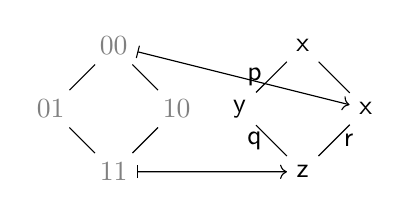
\begin{tikzpicture}[scale=.8]
        \node (zz) at (0,1) {\textcolor{gray}{00}}; \node (zo) at (-1,0)
        {\textcolor{gray}{01}}; \node (oz) at (1,0) {\textcolor{gray}{10}};
        \node (oo) at (0,-1) {\textcolor{gray}{11}}; \draw (zz) -- (zo) --
        (oo) -- (oz) -- (zz);

        \node (zz2) at (3,1) {$\cset{x}$};
        \node (zo2) at (2,0) {$\cset{y}$};
        \node (oz2) at (4,0) {$\cset{x}$};
        \node (oo2) at (3,-1) {$\cset{z}$};

        \draw (zz2) -- (zo2) node[midway,left] {$\cset{p}$};
        \draw (zz2) -- (oz2) node[midway,right] {};
        \draw (oz2) -- (oo2) node[midway,right] {$\cset{r}$};
        \draw (zo2) -- (oo2) node[midway,left] {$\cset{q}$};

        % TODO DRAW EDGE LABELS

        \draw[|->] (zz) -- (oz2);
        \draw[|->] (oo) -- (oo2);
      \end{tikzpicture}
    \end{center}
    \end{column}

    \end{columns}
\end{frame}



\begin{frame}
  \frametitle{CSP solution}

  \hcompcube{\cset{r}}{\cset{p}}{\cset{q}}{\cont{\cset{z}}{\smap{1}}}{\cont{\cset{r}}{\substfour{0}{0}{0}{1}}}{\cont{\cset{p}}{\substfour{0}{1}{0}{1}}}{\cont{\cset{q}}{\substfour{0}{1}{0}{1}}}{\cont{\cset{r}}{\substfour{0}{1}{1}{1}}}{\cont{\phi}{\substfour{00}{10}{01}{11}}} 


\end{frame}






\begin{frame}
  \frametitle{Example}
  \begin{exampleblock}{}
    \textbf{Triangle:}
    
    $\mlist{ \cset{x} : \mlist{} , \cset{y} : \mlist{} , \cset{z} : \mlist{} ,
      \cset{p} : \mlist{ \cset{x}, \cset{y}  } ,
      , \cset{q} : \mlist{ \cset{y}, \cset{z} }
      , \cset{r} : \mlist{ \cset{x}, \cset{z} }
      , \cset{\phi} : \mlist{ \cset{p} , \cset{r} ,
        \cont{\cset{x}}{\oneconst}, \cset{q} }
    }$
  \end{exampleblock}

  \begin{columns}
    \begin{column}{.5\textwidth}
      \hcompcubesmall{\cset{p}}{\cset{p}}{\cset{q}}{\cset{q}}{X_{1,\izero}}{X_{2,\izero}}{X_{1,\ione}}{X_{2,\ione}}{X_\text{B}}
    \end{column}
    \begin{column}{.5\textwidth}
      $D_{1,0} = \{ \cont{\cset{p}}{\substfour{0}{0,1}{0}{1}} \}$
      
      $D_{1,1} = \{ \cont{\cset{q}}{\substfour{0}{0,1}{0}{1}} \}$

      $D_{1,0} = \{ \cont{\cset{p}}{\substfour{0}{0,1}{0}{1}} \}$
      
      $D_{1,1} = \{ \cont{\cset{q}}{\substfour{0}{0,1}{0}{1}} \}$

    \end{column}
  \end{columns}

  $D_{B} = \{ \cont{\cset{x}}{\substfour{()}{()}{()}{()}} , ... ,
  \cont{\cset{p}}{\substfour{0,1}{0,1}{0,1}{0,1}}, ... , \cont{\phi}{\substfour{00,01,10,11}{00,01,10,11}{00,01,10,11}{00,01,10,11}} \}$
\end{frame}

\begin{frame}
  \frametitle{CSP solution}

  \hcompcube{\cset{p}}{\cset{p}}{\cset{q}}{\cset{q}}{\cont{\cset{p}}{\substfour{0}{1}{0}{1}}}{\cont{\cset{p}}{\substfour{0}{1}{0}{1}}}{\cont{\cset{q}}{\substfour{0}{0}{0}{1}}}{\cont{\cset{q}}{\substfour{0}{0}{0}{1}}}{\cont{\cset{p}}{\substfour{0}{1}{1}{1}}}

\end{frame}

\backupend

\end{document}


%%% Local Variables: 
%%% coding: utf-8
%%% mode: latex
%%% TeX-engine: xetex
%%% End: 
